\documentclass{article}
\usepackage{amsmath}
\title{Night Light}
\author{wandyezj}

\usepackage{comment}
\usepackage[yyyymmdd]{datetime}
\renewcommand{\dateseparator}{--}


\usepackage{verbatim}

\usepackage[margin=0.5in]{geometry}

\usepackage{enumitem}

\usepackage{listings}
\usepackage{color}

\definecolor{dkgreen}{rgb}{0,0.6,0}
\definecolor{gray}{rgb}{0.5,0.5,0.5}
\definecolor{mauve}{rgb}{0.58,0,0.82}

	\lstset{frame=tb,
	language=Java,
	aboveskip=3mm,
	belowskip=3mm,
	showstringspaces=false,
	columns=flexible,
	basicstyle={\small\ttfamily},
	numbers=none,
	numberstyle=\tiny\color{gray},
	keywordstyle=\color{blue},
	commentstyle=\color{dkgreen},
	stringstyle=\color{mauve},
	breaklines=true,
	breakatwhitespace=true,
	tabsize=3
}


\usepackage{graphicx}
%Path in Windows format:
\graphicspath{ {images/} }

\usepackage{subfig}

\usepackage{hyperref}
\hypersetup{
	colorlinks=true,
	linkcolor=blue,
	filecolor=magenta,      
	urlcolor=cyan,
}

\begin{document}
	\maketitle
	\tableofcontents
	
	
	
	\clearpage
	
	\section{Overview}
	% (i) provides an overview of your night light; 
	
	Youtube Video Link Hardware: \href{https://www.youtube.com/watch?v=zhsaB9KtgVE}{https://www.youtube.com/watch?v=zhsaB9KtgVE}\newline
	Youtube Video Link Software: \href{https://youtu.be/YWPwPMCAAq8}{https://youtu.be/YWPwPMCAAq8}\newline
	Github Link: \href{https://github.com/wandyezj/night_light}{https://github.com/wandyezj/night\_light}\newline
	\newline
	Code Overview:
	\newline
	AndroidBLEBasic - Main Android application code
	\newline
	nightlight - UI draft
	\newline
	arduino\_lightlight - hardware code
	\newline
	\newline
	
	The night light comes in a case ideal for store shelves. A cotton ball is used for light diffusion (\ref{fig:hardware}).
	\newline
	A manual slide bar allows adjustment of the color and turning off (\ref{fig:hardware_board_layout}). 
	\newline
	A light sensor controls the brightness inverse of the light level (\ref{fig:hardware_board_layout}).
	\newline
	An android application allows for remote control of the color after connecting via bluetooth (\ref{fig:android_app}).
	\newline
	The application may change the light color via slide bar (\ref{fig:android_app_slidebar_select}) or via tilting of the phone (\ref{fig:android_app_gyroscope_select}).
	
	
	% controls hardware, and software

	\begin{figure}[h!]
		\centering
		\hfill
		\subfloat[Board]{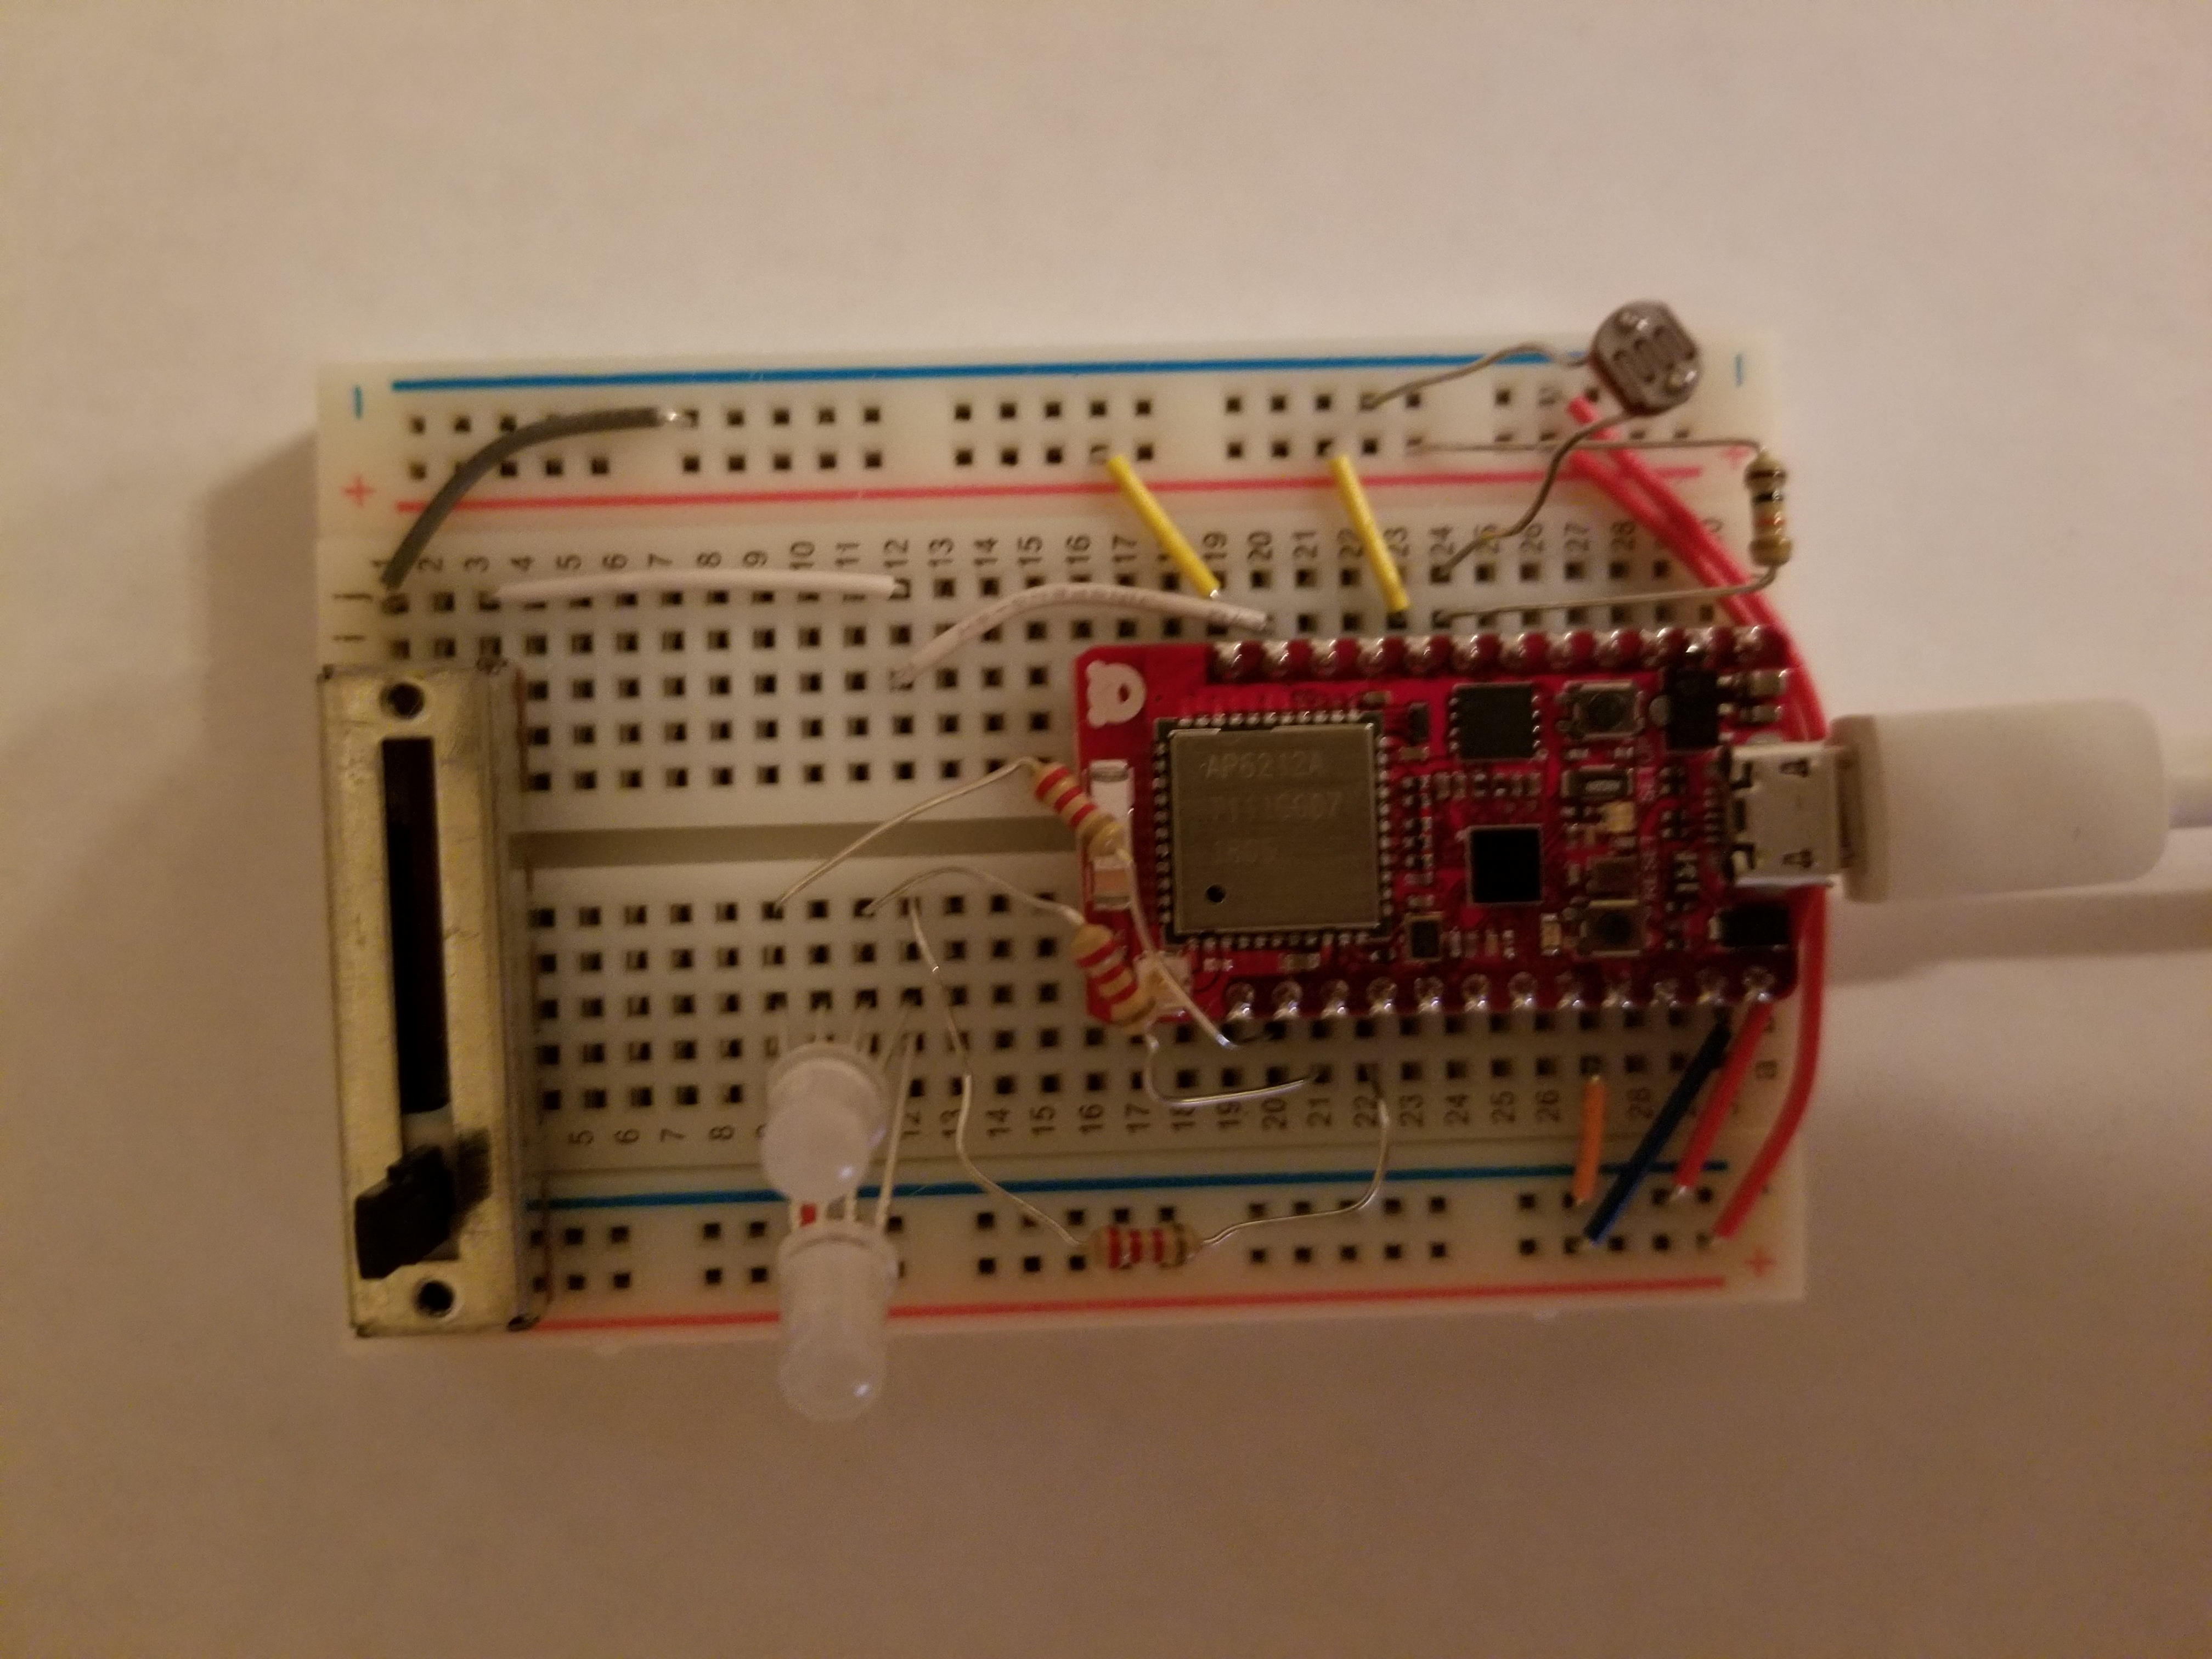
\includegraphics[width=0.5\textwidth]{hardware_board_layout}\label{fig:hardware_board_layout}}
		\hfill
		\subfloat[Eclosure]{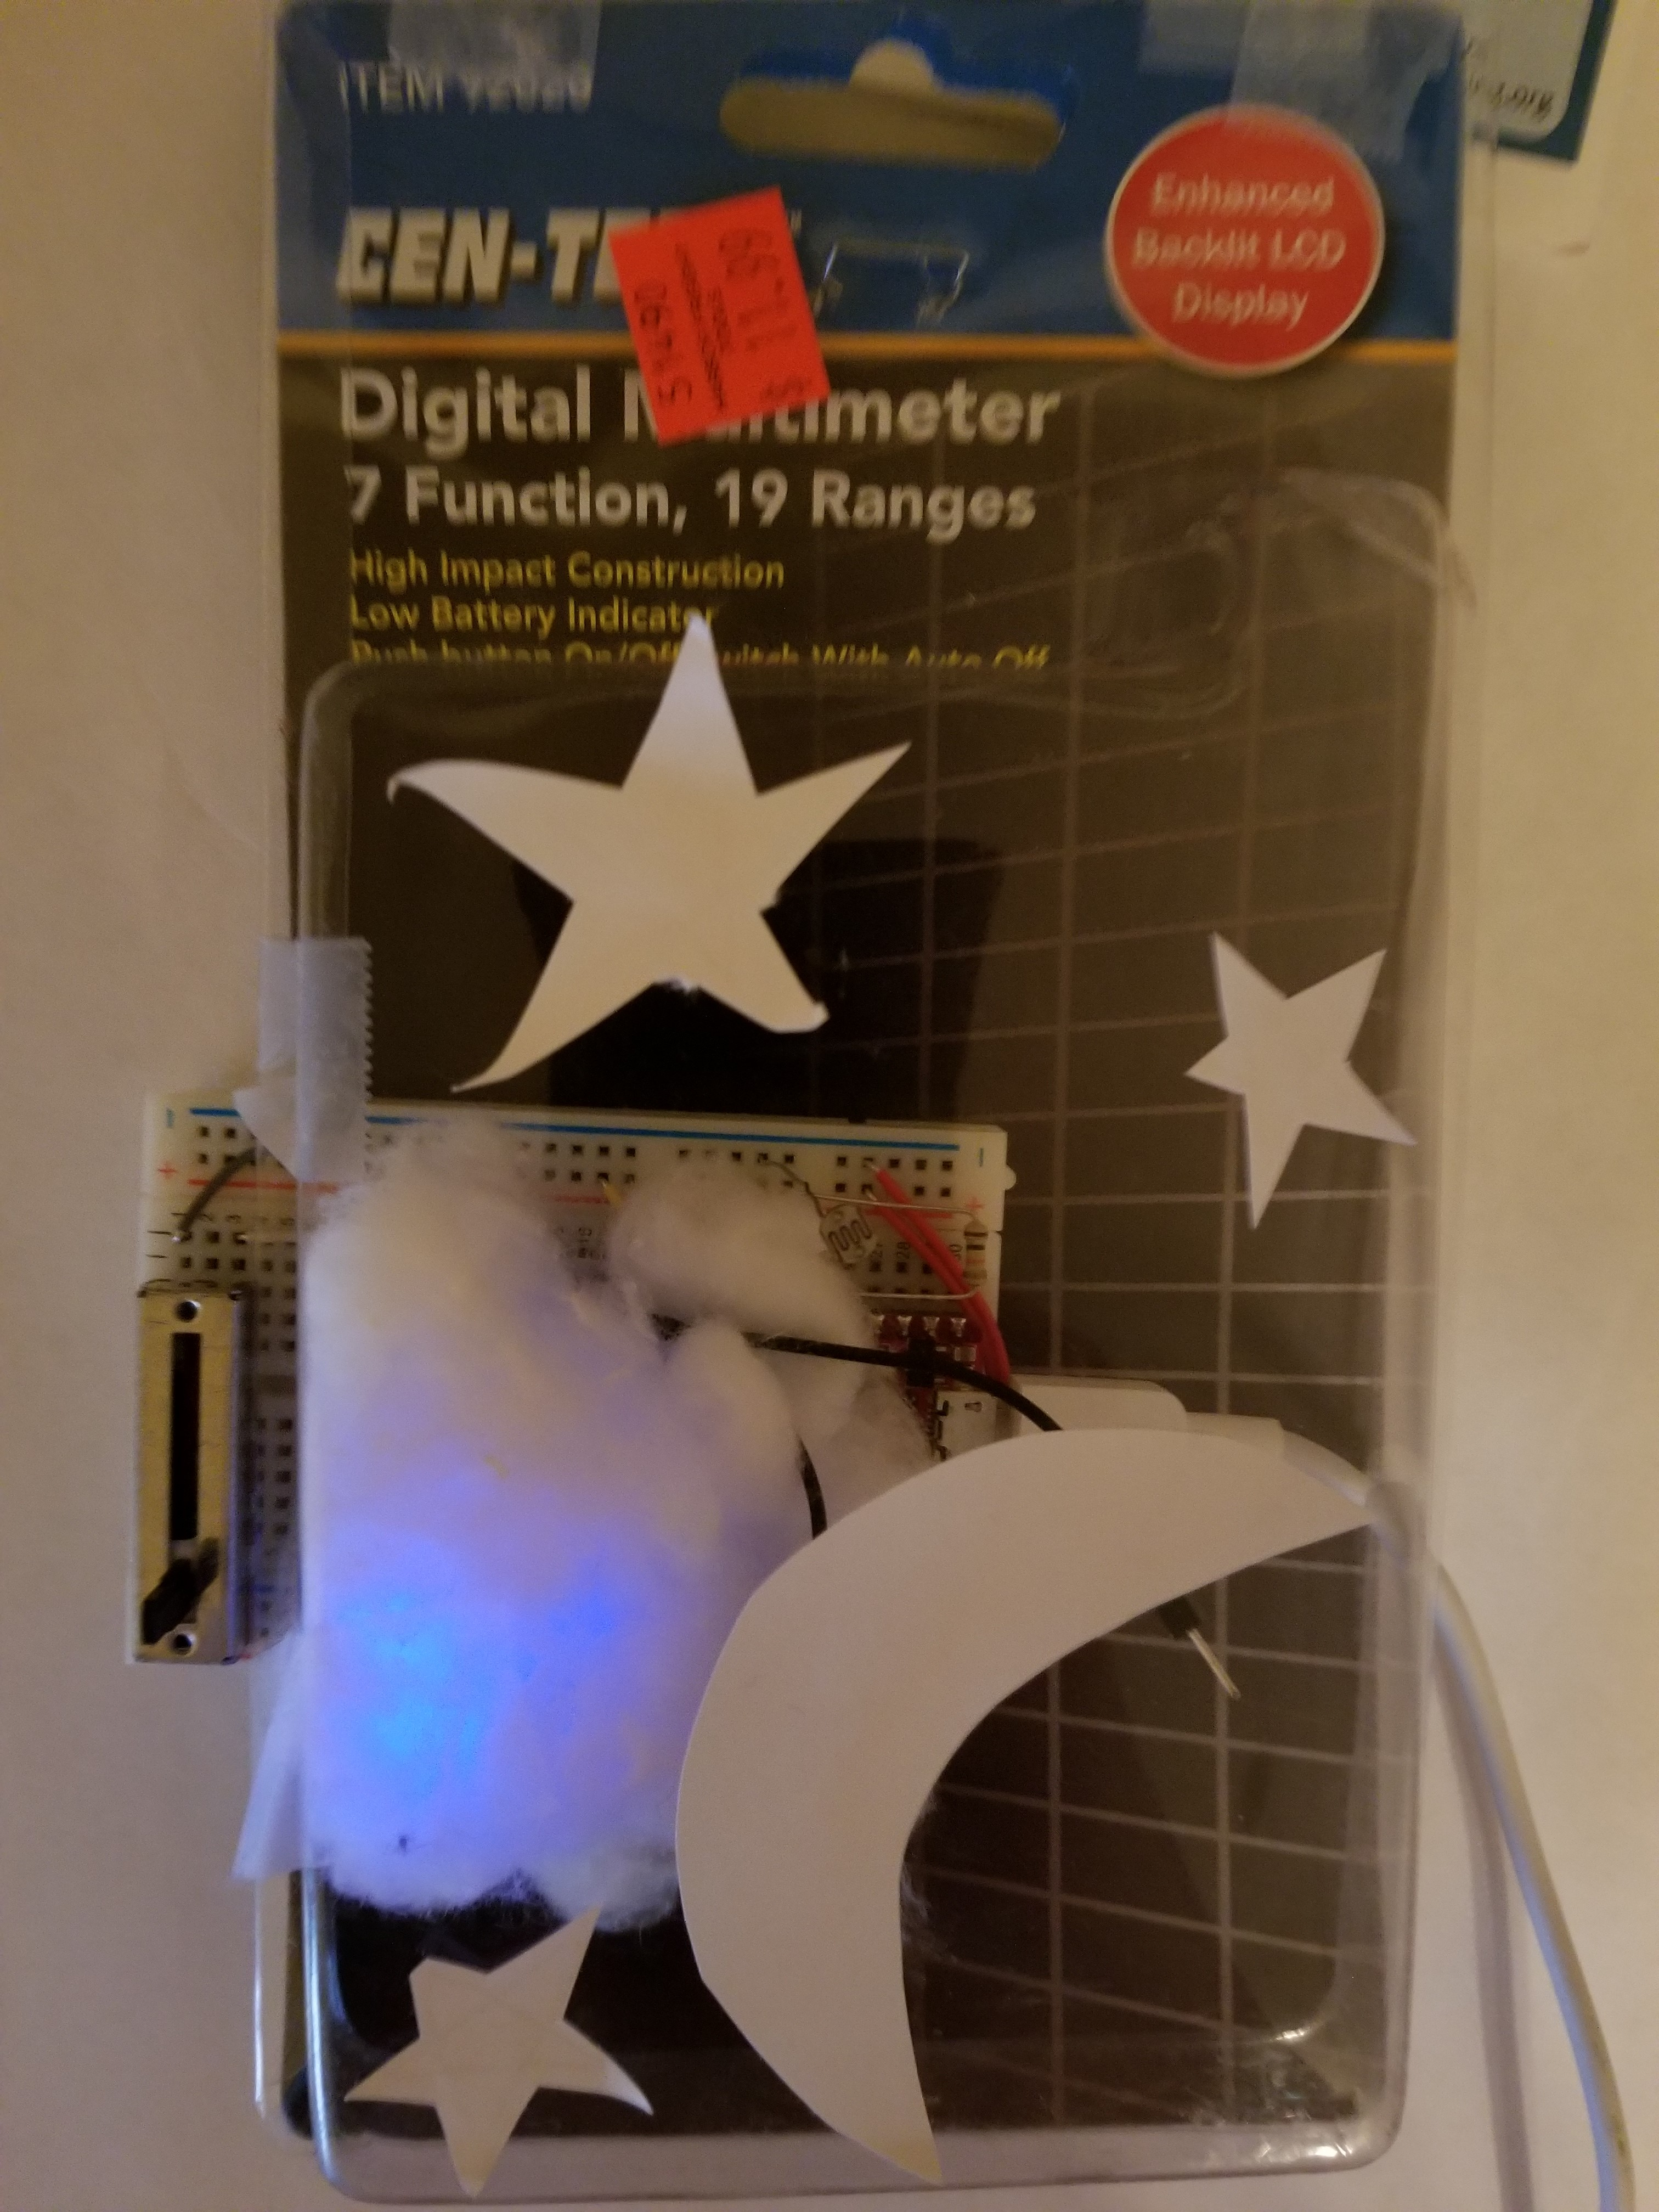
\includegraphics[width=0.4\textwidth]{hardware_package}\label{fig:hardware_package}}
		\hfill
		\hfill
		\caption{Hardware}
		\label{fig:hardware}
	\end{figure}

	\begin{figure}[h!]
		\centering
		\hfill
		\subfloat[Android App Layout]{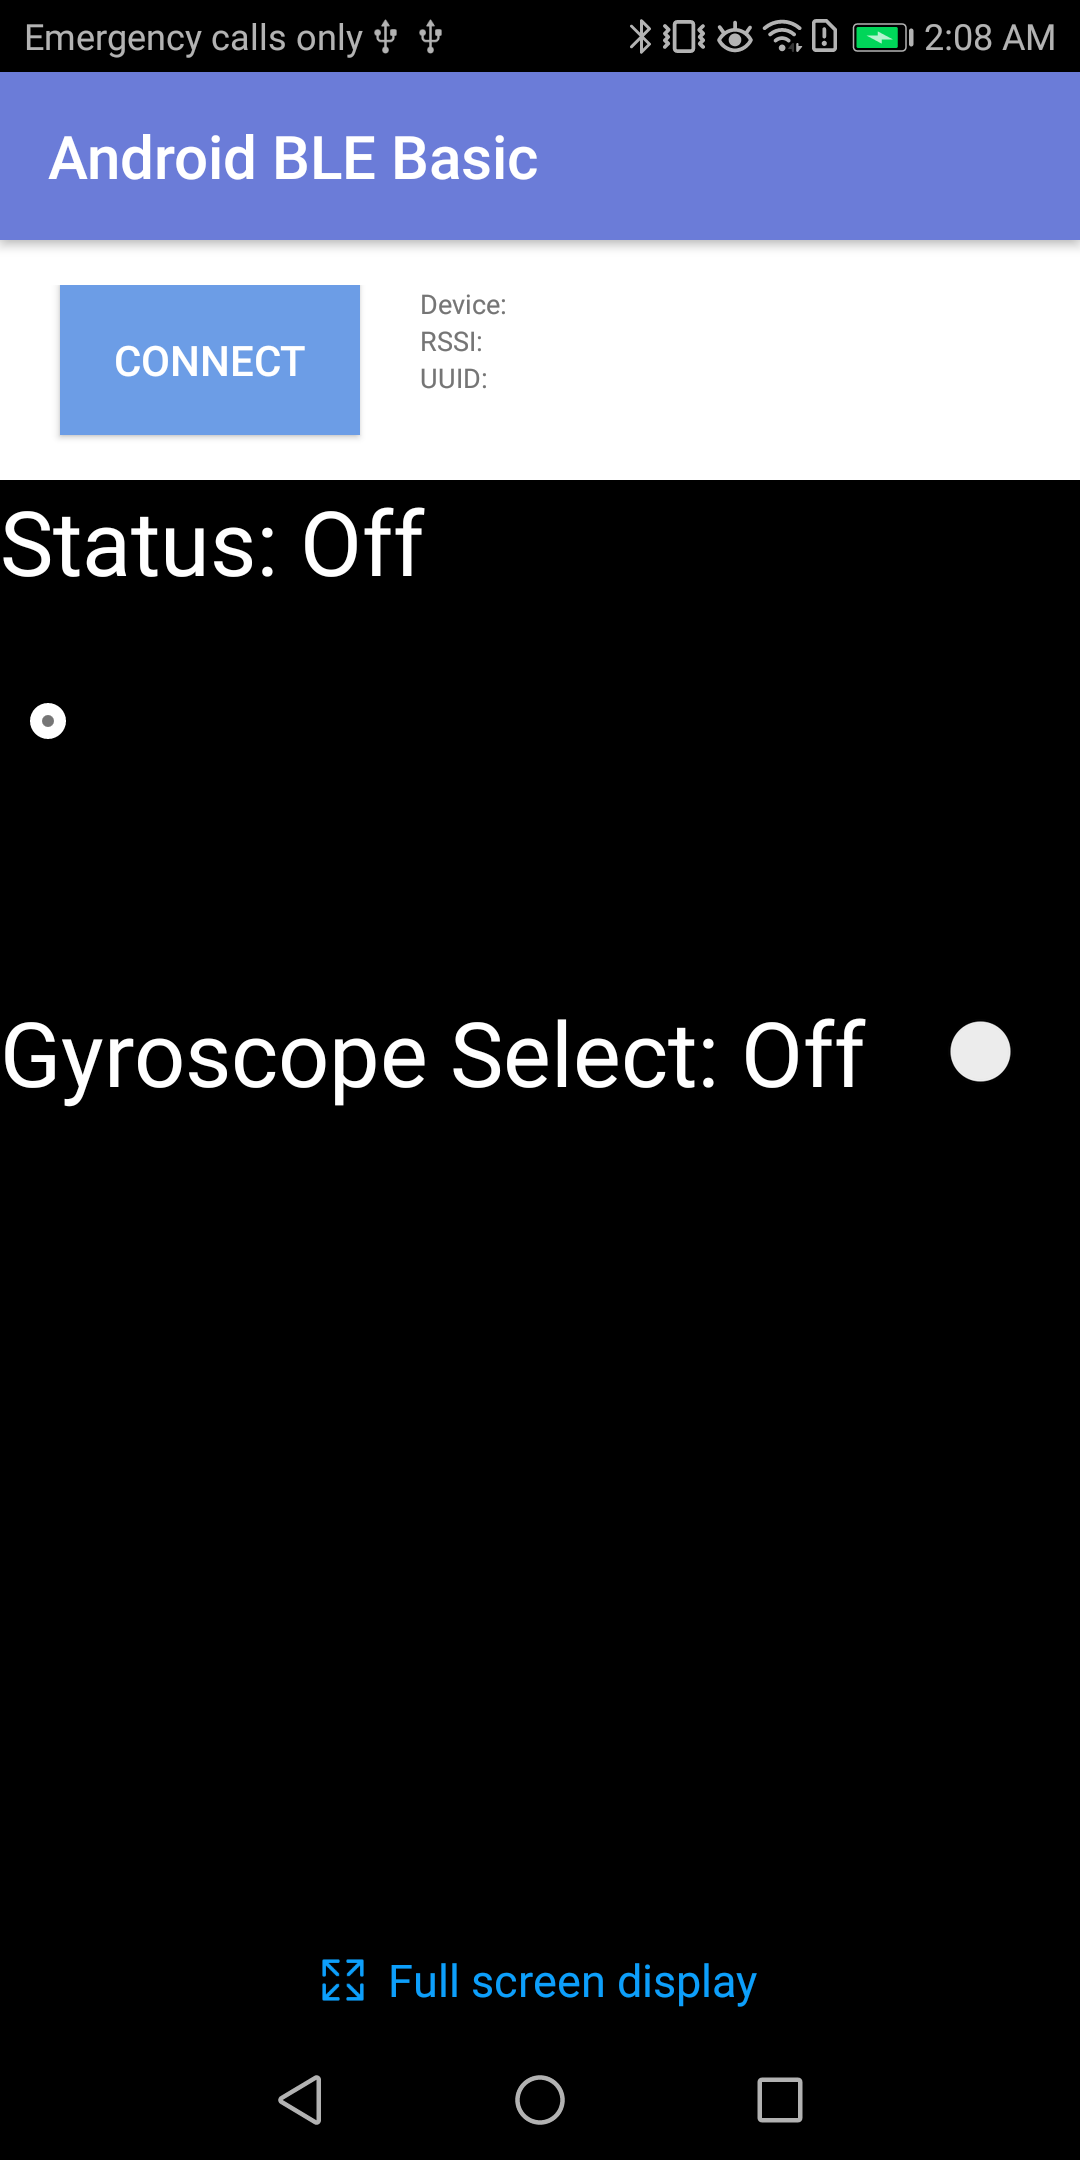
\includegraphics[width=0.2\textwidth]{android_app_layout}\label{fig:android_app_layout}}
		\hfill
		\subfloat[Android App Connected]{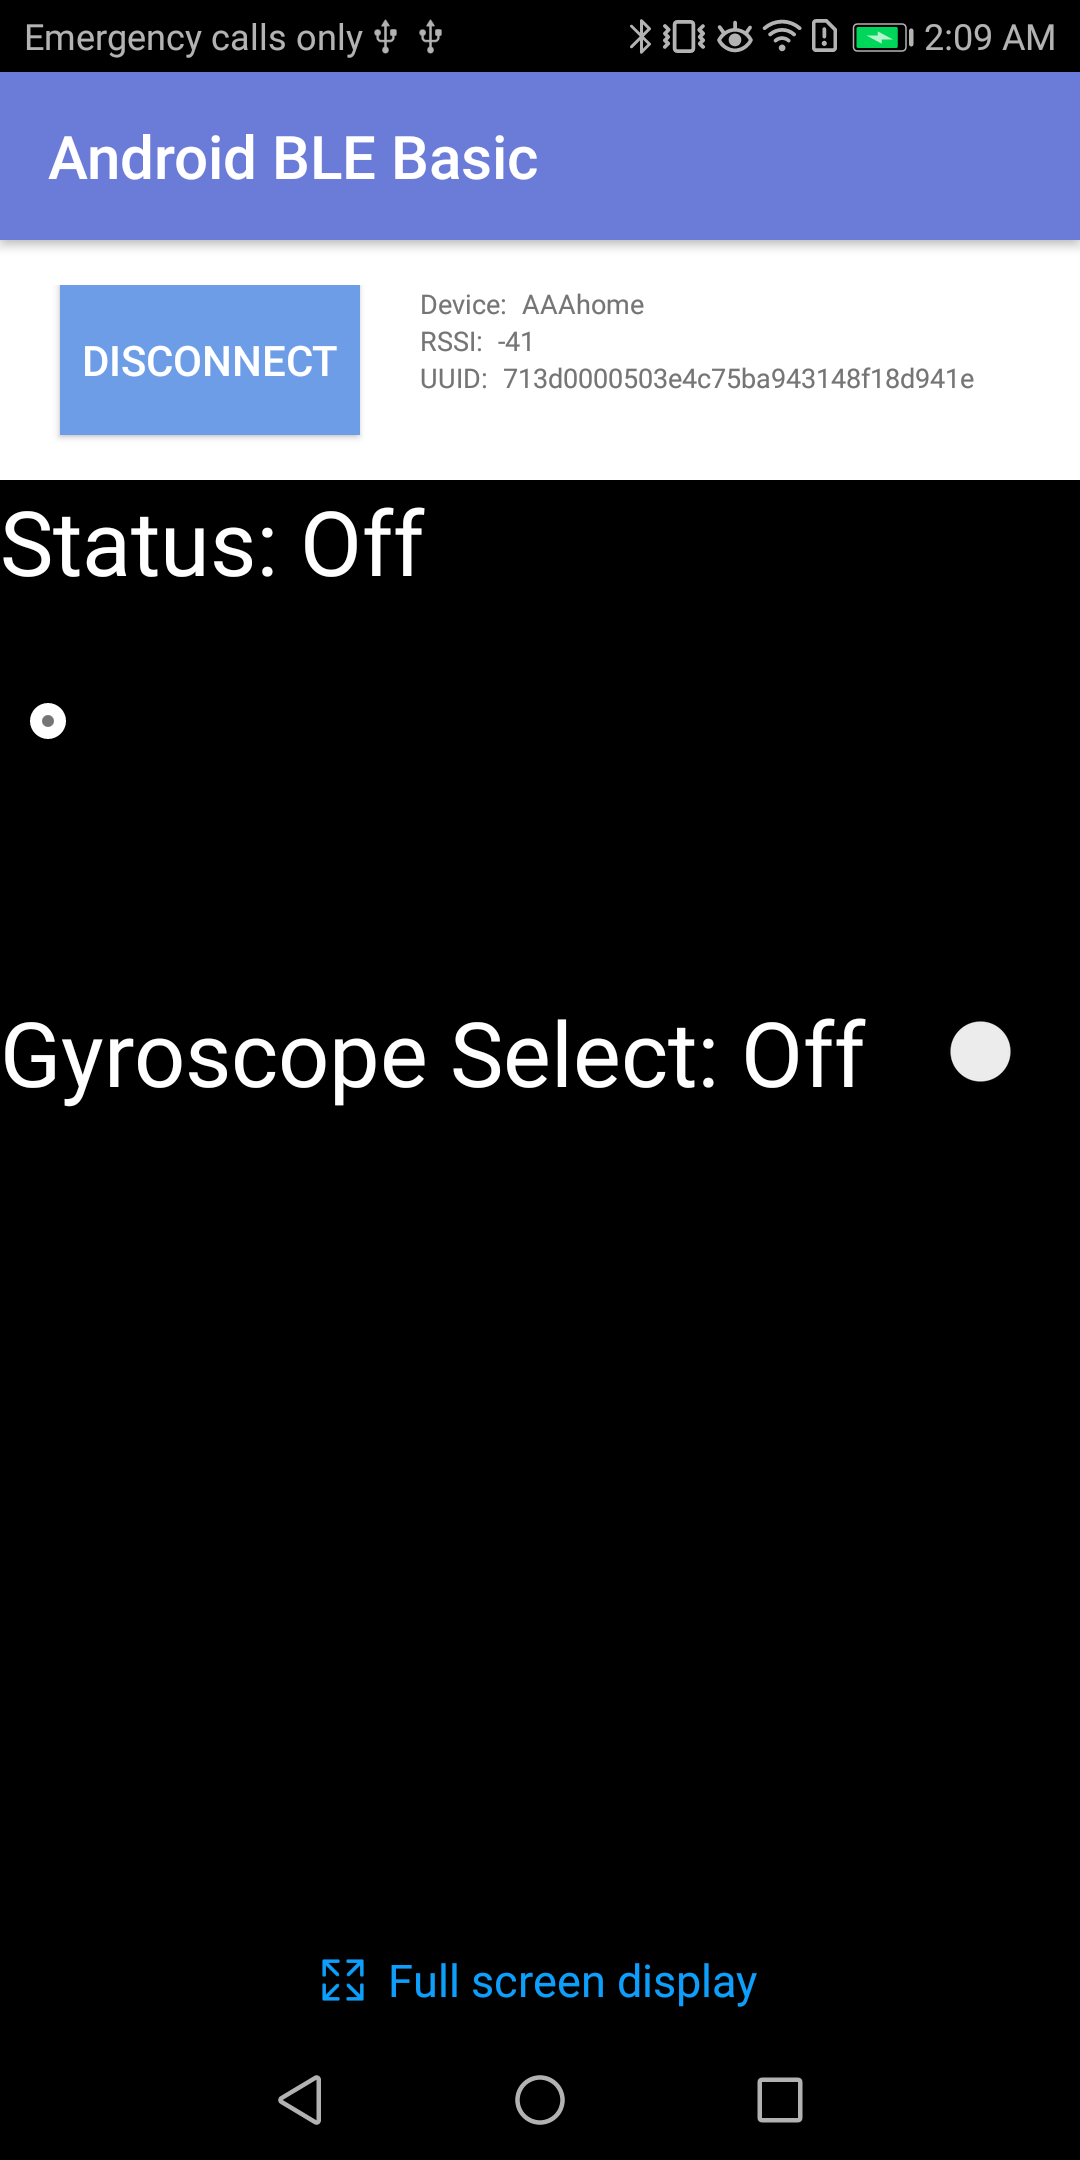
\includegraphics[width=0.2\textwidth]{android_app_connected}\label{fig:android_app_connected}}
		\hfill
		\subfloat[Slidebar Select]{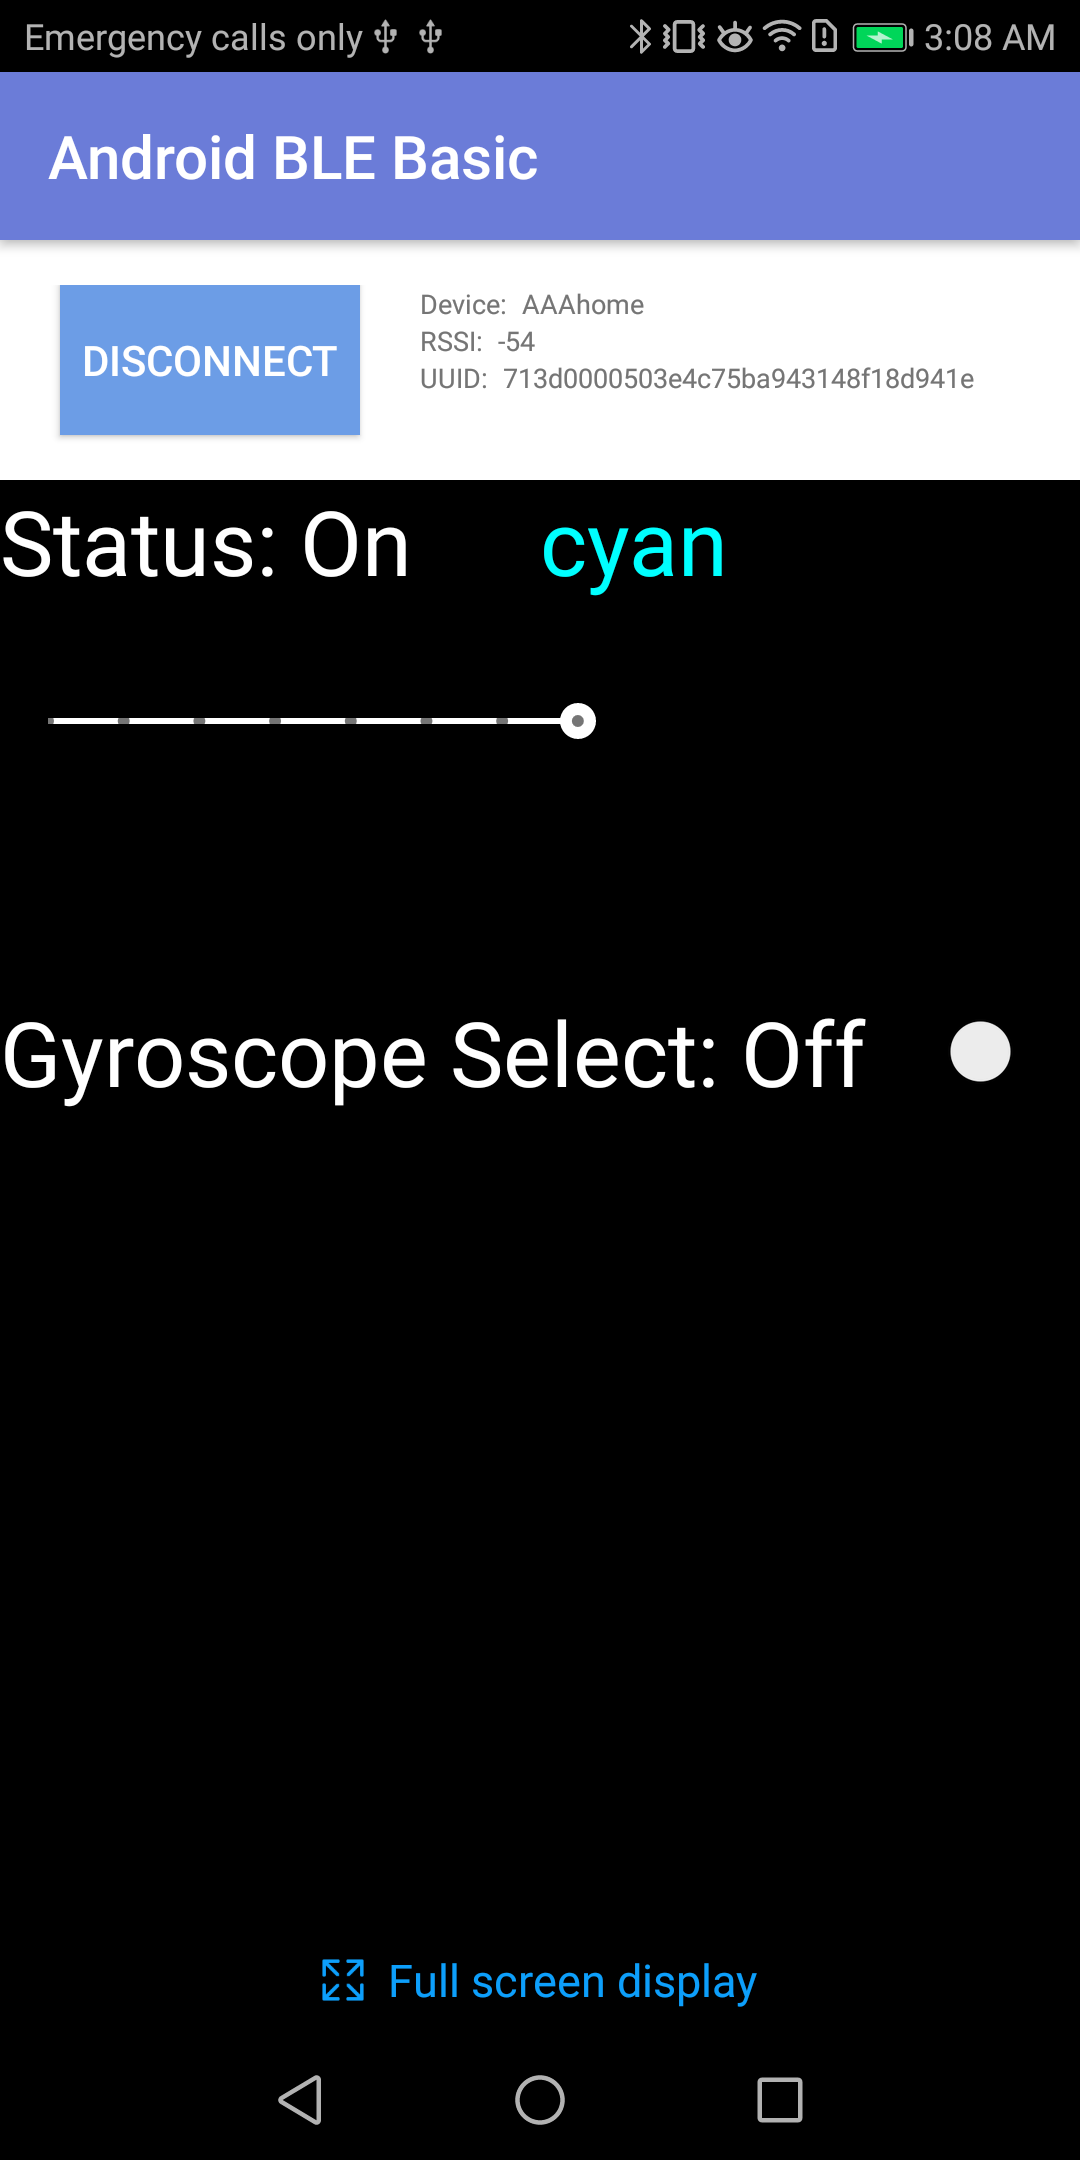
\includegraphics[width=0.2\textwidth]{android_app_slidebar_select}\label{fig:android_app_slidebar_select}}
		\hfill
		\subfloat[Gyroscope Select]{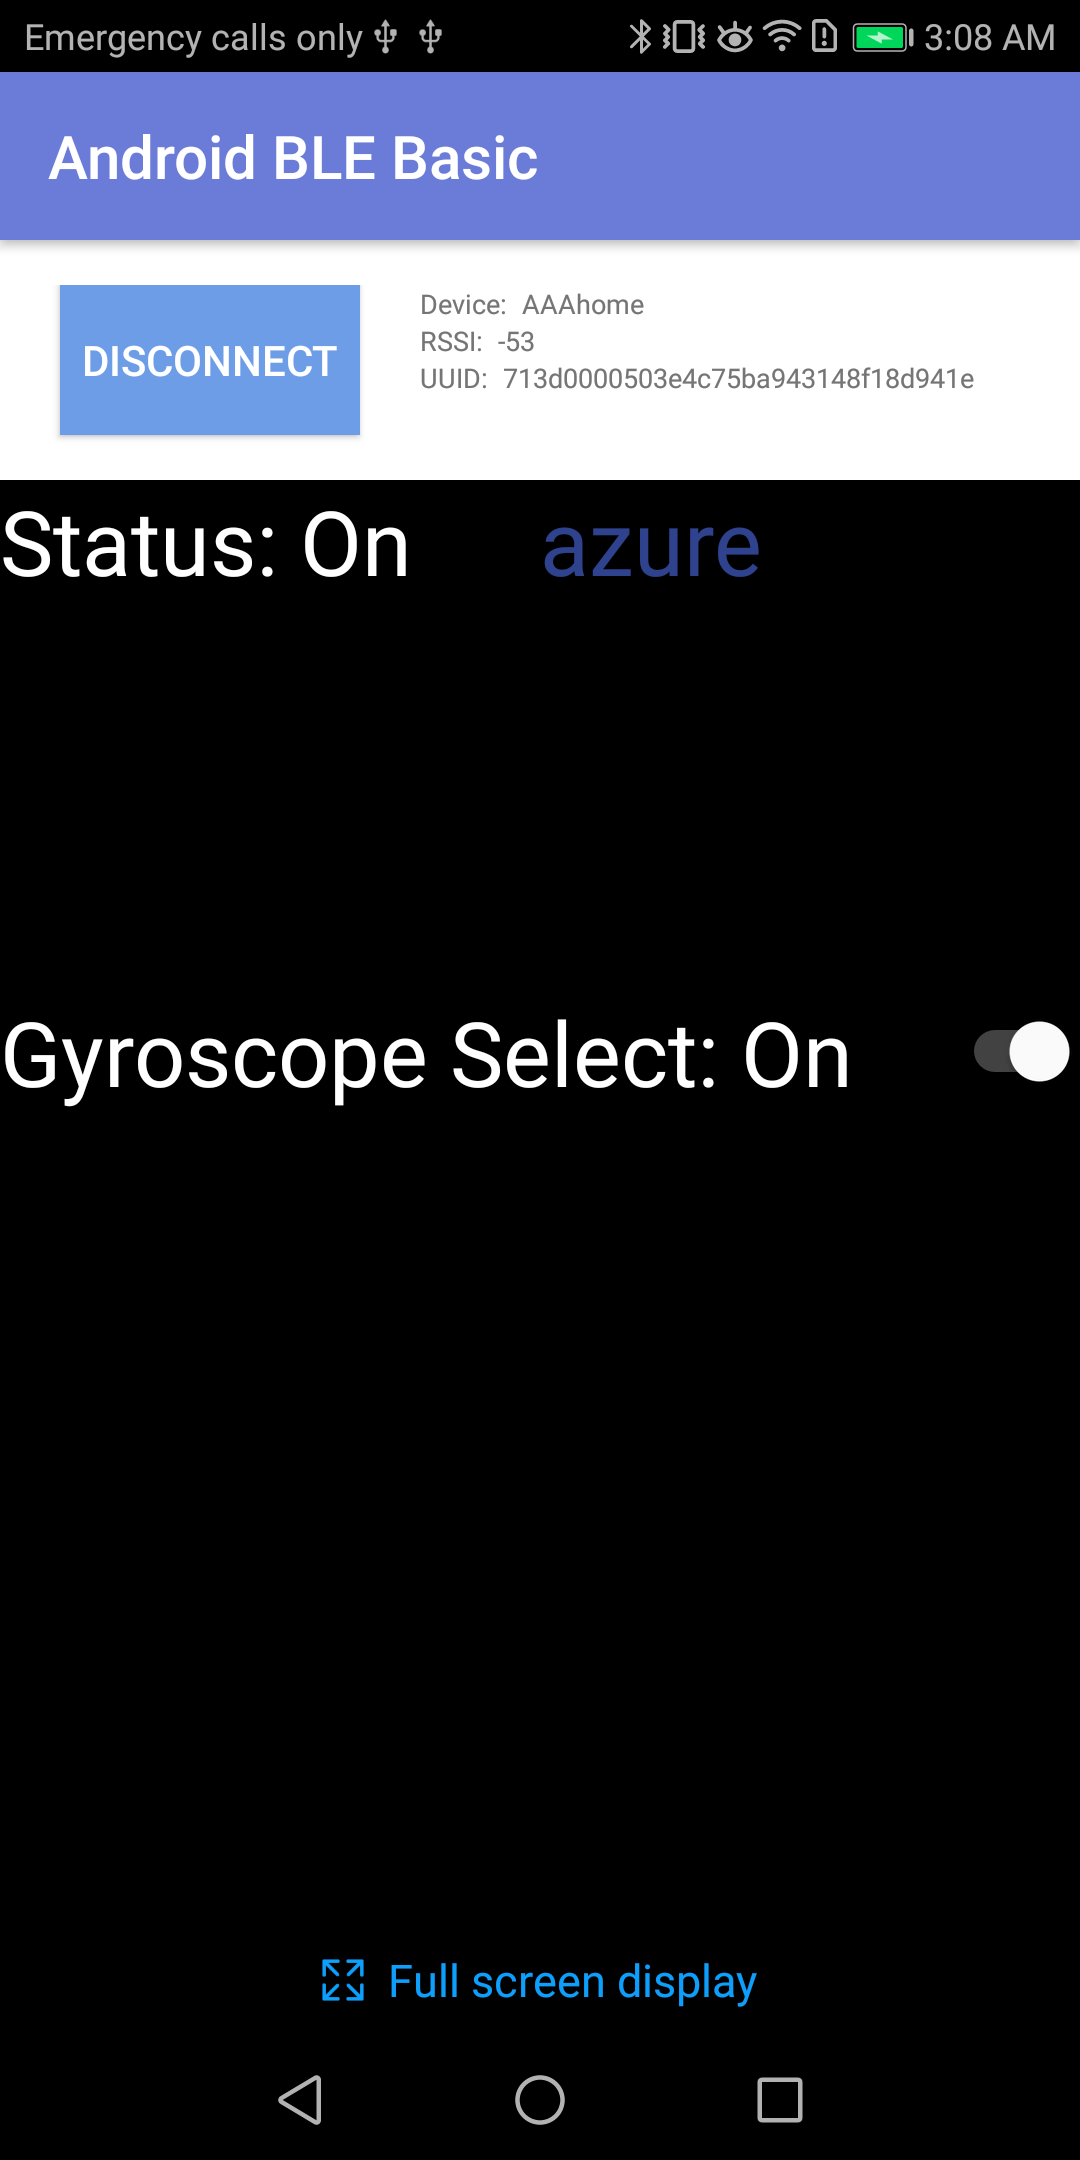
\includegraphics[width=0.2\textwidth]{android_app_gyroscope_select}\label{fig:android_app_gyroscope_select}}
		\hfill
		\hfill
		\caption{Android App Basics}
		\label{fig:android_app}
	\end{figure}
	
	\begin{figure}[h!]
		\centering
		\hfill
		\subfloat[Bluetooth Color Select]{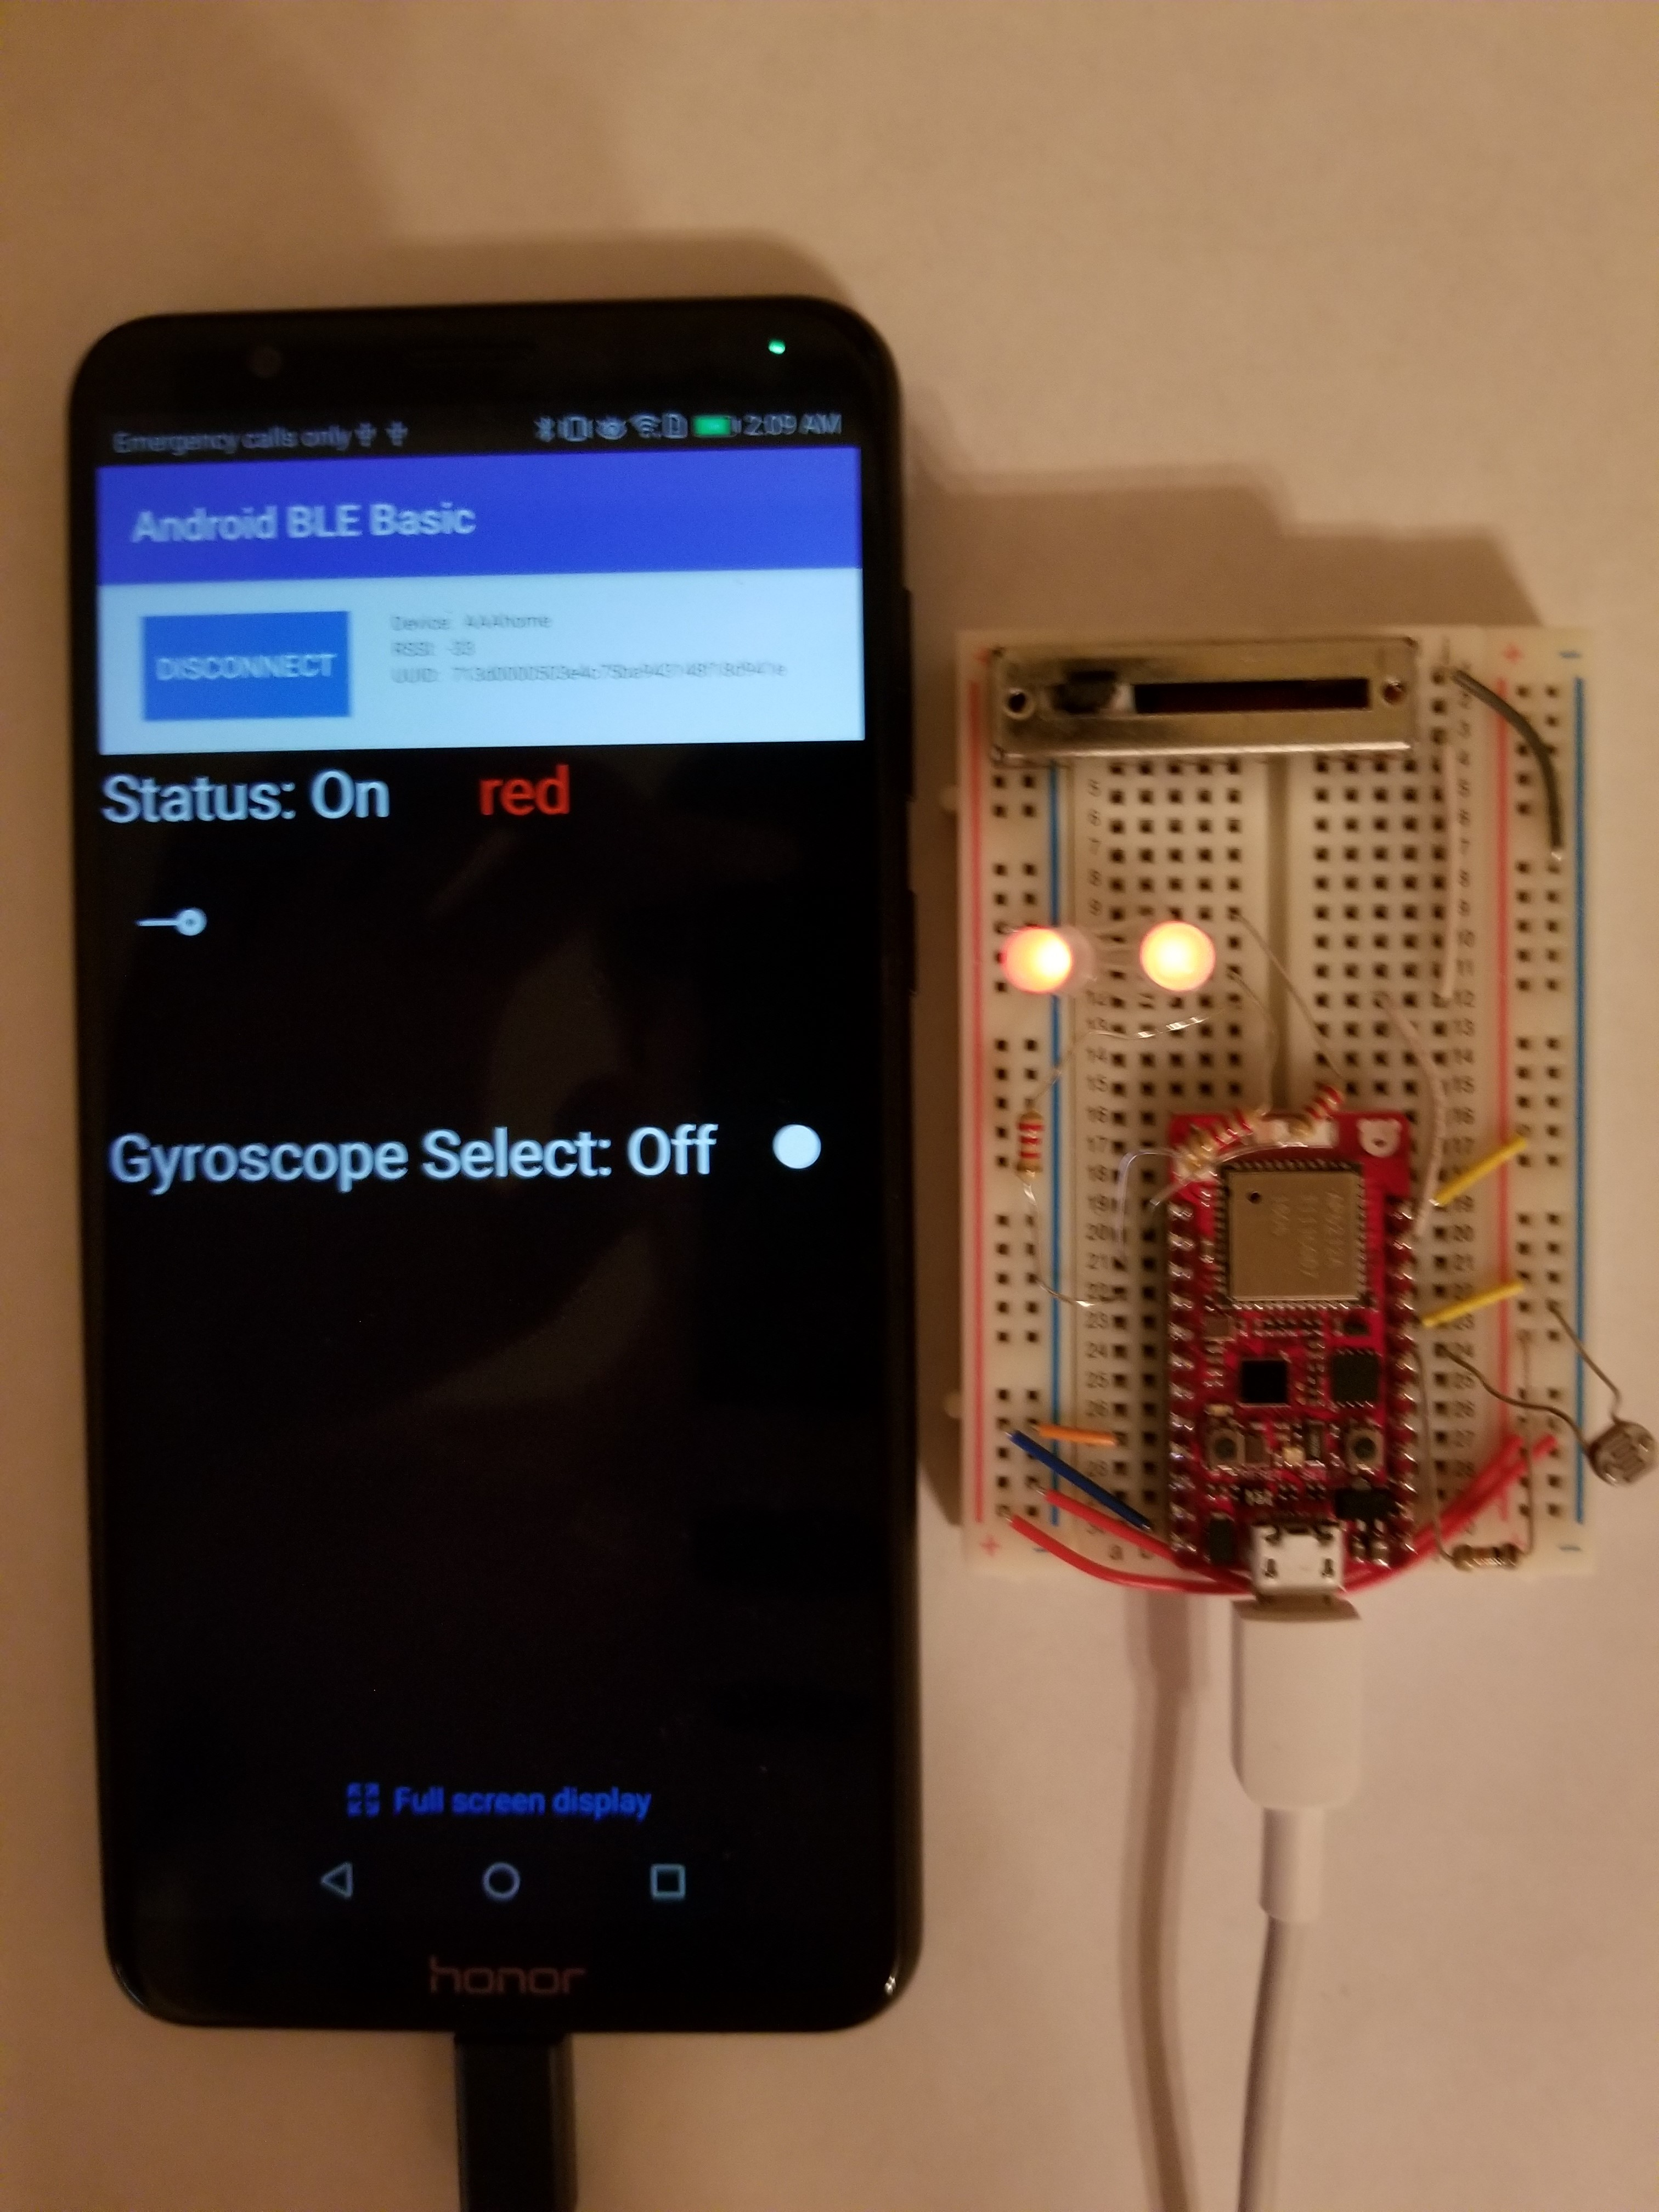
\includegraphics[width=0.4\textwidth]{bluetooth_color_select}\label{fig:bluetooth_color_select}}
		\hfill
		\subfloat[Bluetooth Blink]{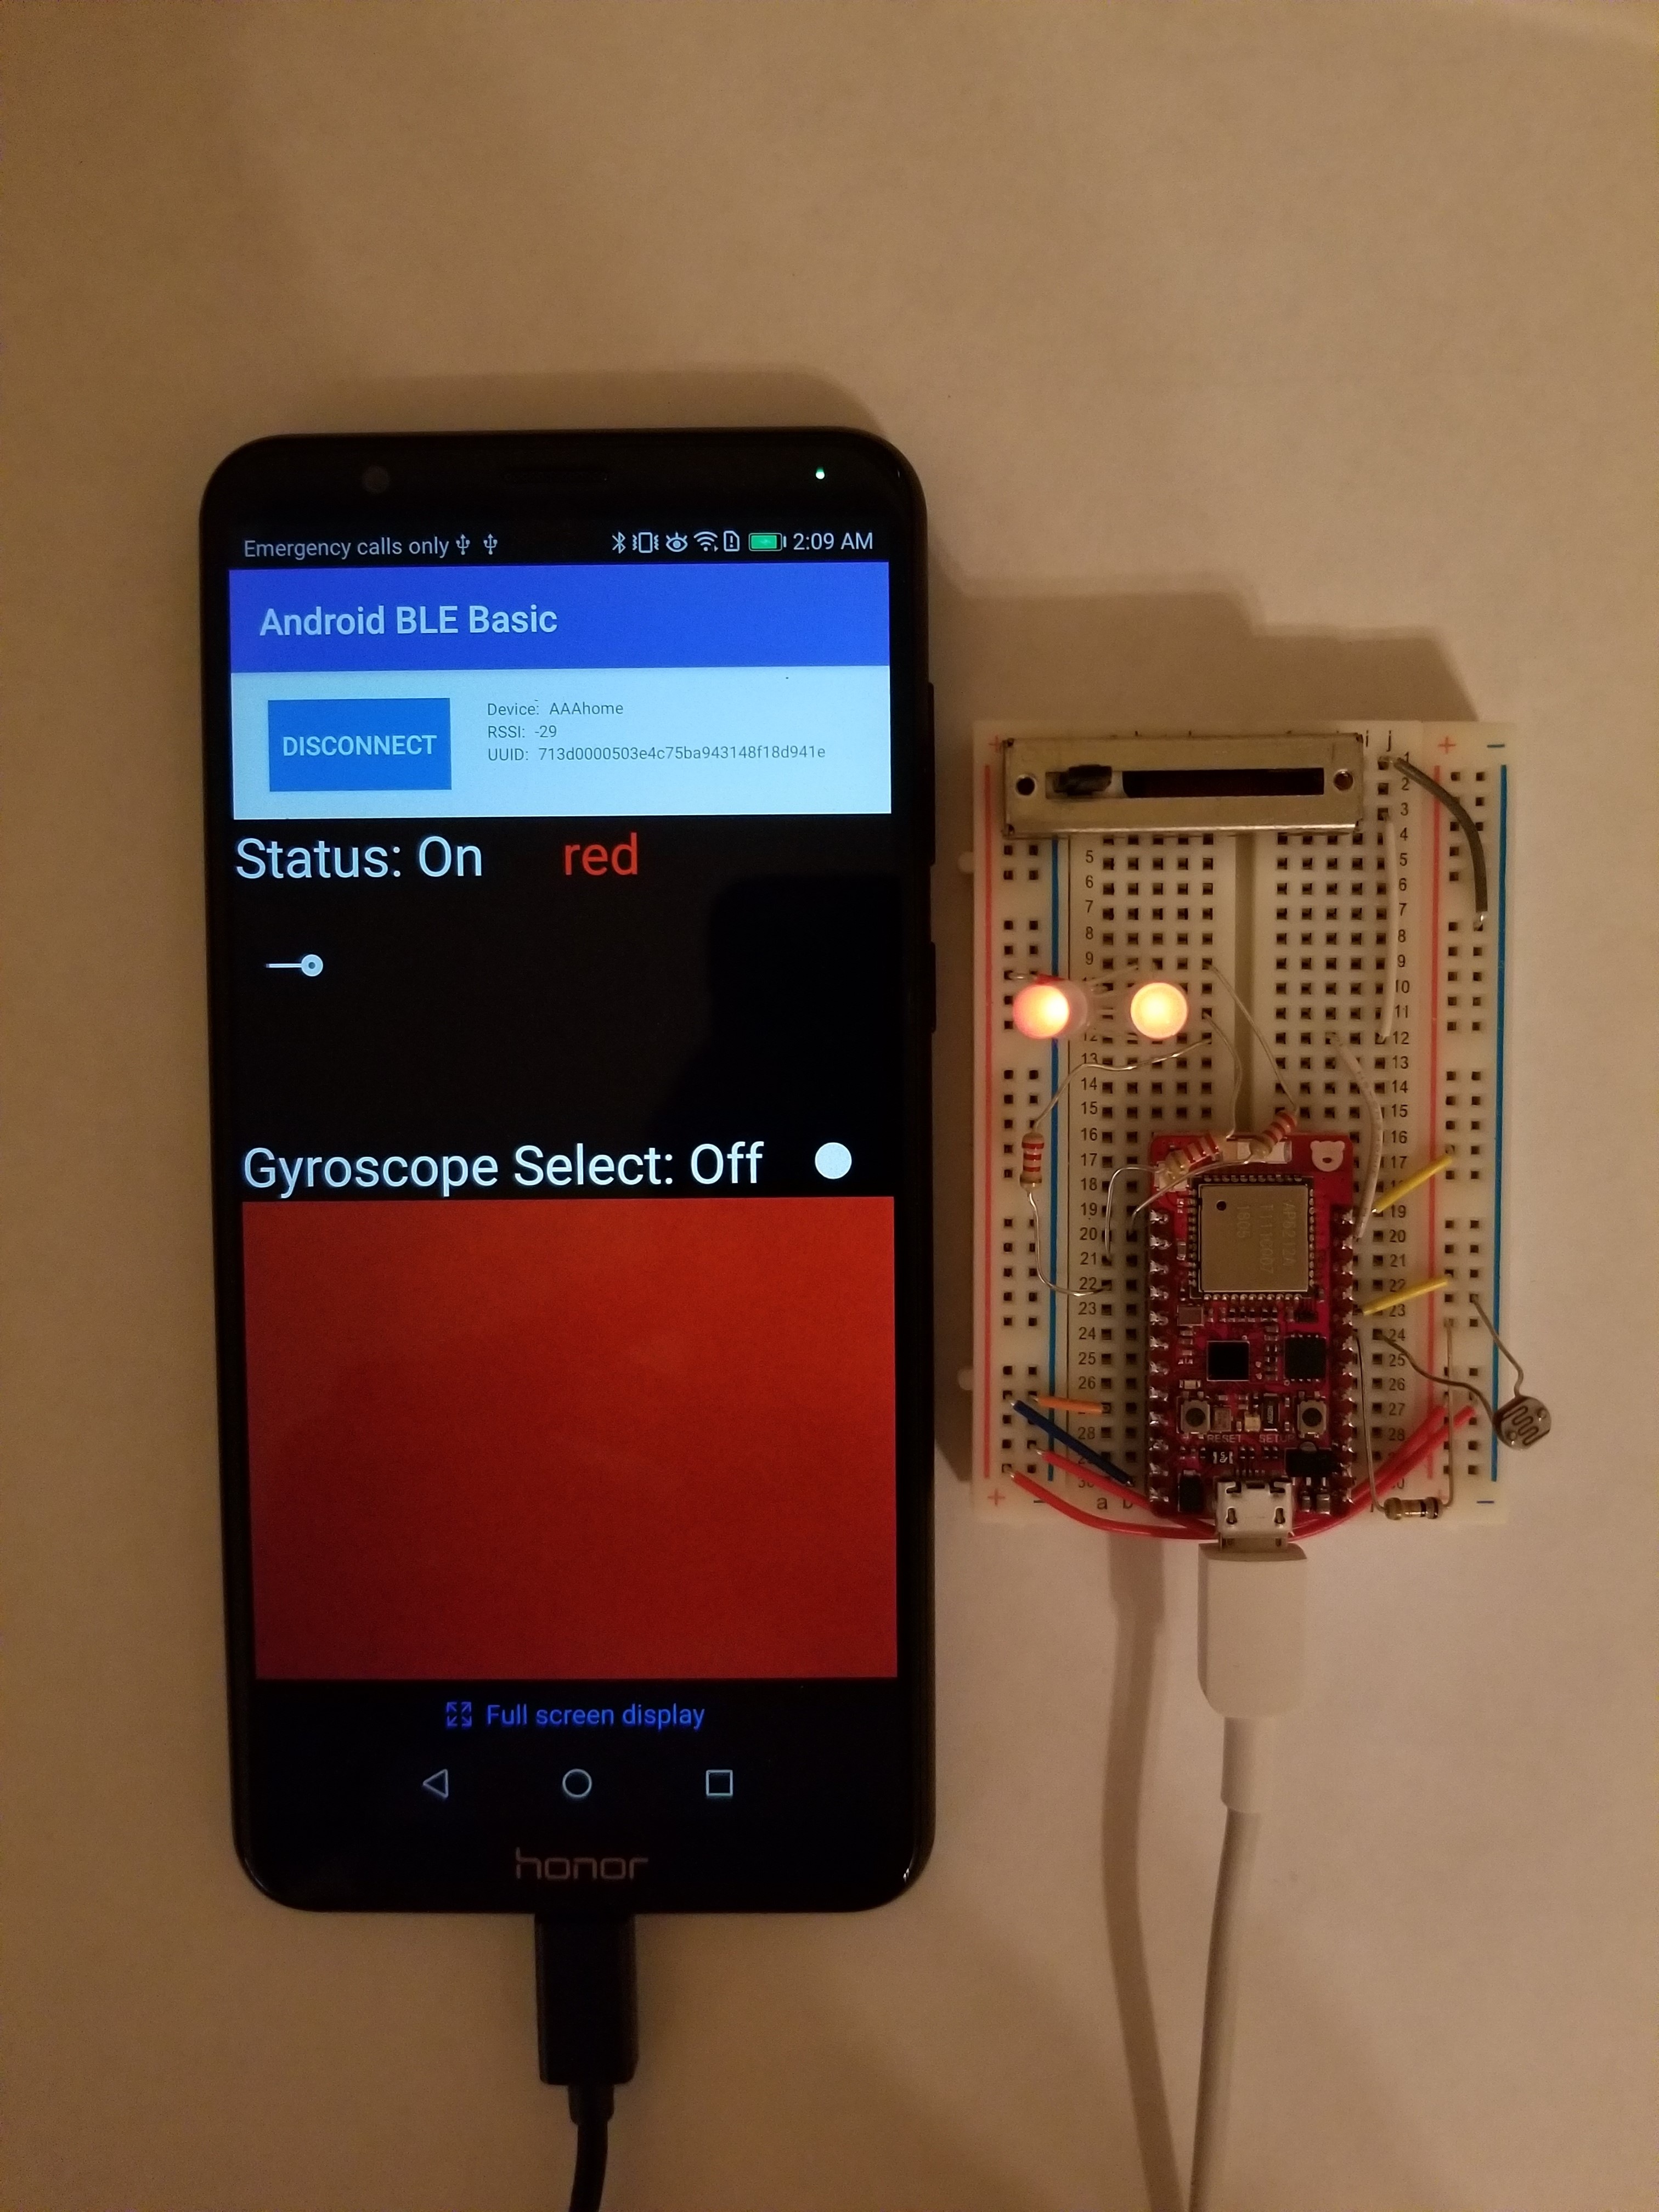
\includegraphics[width=0.4\textwidth]{blink_on}\label{fig:blink_on}}
		\hfill
		\hfill
		\caption{Software Control}
		\label{fig:software_control}
	\end{figure}
	
	\clearpage
	\section{Creative Feature}
	% (ii) describes your creative feature; 
	
	% hardware override
	% Blinking
	% filtering for hardware input
	% instant reaction with loop timing
	
	The creative features are:
	\begin{itemize}
		\item A double tap at the bottom of the android app toggles the lights blinking functionality. 
		\item The screen blinks when blinking action is on. Mid-blink:(\ref{fig:bluetooth_color_select})
		\item Hardware inputs reading are filtered to avoid random color changes.
		\item Instant reaction with hardware timing, there are no 'perceived delays' for actions taken by users.
		\item A change in the physical switch always overrides software changes.
	\end{itemize}

	
	
	\section{Challenges}
	% (iii) enumerates key struggles and challenges; 
	
	\begin{itemize}
		\item Working with a physical system and software. Not knowing which has the issue.
		\item Having wires everywhere makes it hard to see the circuit.
		\item Constructing an enclosure (physical crafts are difficult, and it interferes with debugging)
		\item Bluetooth, I still don't understand this protocol.
		\item Organizing the arduino code, should have broken it into multiple files.
	\end{itemize}
	
	\section{Reflection}
	%(v) reflect on what you learned.
	%You should include as many images as you want (at least one) that helps explain your night light. Images are free. You need not write in prose (you can bullet point the entire report).
	
	\begin{itemize}
		\item Doing a better job of organizing the Arduino code would have been helpful.
		\item Electronic sensors do not have constant readings and require filtering.
		\item Arduino central loop model requires timing to simulate multiple actions.
		\item HSL and HSV would have been cooler than a fixed color selection.
		\item fritzing is a cool program that could have been used to plan circuits.
		\item There are a lot of different micro controllers with various costs, sizes, and ease of use.
		\item There is an advantage to having easy to program hardware.
		\item Organizing wires is super helpful for debugging.
	\end{itemize}
	
\end{document}